\fenicschapter{Quadrature Representation of Finite Element Variational Forms}
              {Quadrature Representation of Finite Element Variational Forms}
              {Kristian B. \O{}lgaard and Garth N. Wells}
              {oelgaard-2}

%------------------------------------------------------------------------------
This chapter addresses the conventional runtime quadrature approach for the
numerical integration of local element tensors associated with finite element
variational forms, and in particular automated optimisations
which can be performed to reduce the number of floating point operations.
An alternative to the runtime quadrature approach is the tensor
representation, as presented in
Chapter~[logg-4], and both the quadrature and tensor approaches are
implemented in \ffc{} (see Chapter~[logg-1]).
We discuss in this chapter four strategies for optimising the quadrature
representation for
runtime performance of the generated code and show that optimisation
strategies lead to a dramatic improvement in runtime performance
over a naive implementation.
It may seem superfluous to have two different methods for
representing variational forms implemented in the same piece of software, but
we will examine aspects of the quadrature and tensor approaches for different
equations, and this will motivate the desirability of being able to choose between
the two representations.
%
%------------------------------------------------------------------------------
\section{Standard quadrature representation}
\label{oelgaard-2:sec:standard_quadrature_representation}
%
To illustrate the standard quadrature representation and optimisations
implemented in \ffc{} we consider the bilinear form for the weighted Laplace
operator $-\nabla \cdot (w \nabla u)$, where $u$ is the unknown and $w$ is
a prescribed coefficient.
The bilinear form of the variational problem for this equation reads
%
\begin{equation}
  a\brac{v, u} = \int_{\Omega} w \nabla v \cdot \nabla u \dx.
\label{oelgaard-2:eq:weightedlaplacian}
\end{equation}
%
Although \ffc{} supports the use of `quadrature functions', that can be
evaluated directly at quadrature points, we assume that all functions in the
following, including the coefficient function $w$, come from the same finite
element function, namely
%
\begin{equation}
  V_{h} = \bracc{v \in H^{1}\brac{\Omega}: \ v\vert_K \in P_{k}\brac{K}
   \forall K \in \mathcal{T}},
\label{oelgaard-2:eq:space_H1}
\end{equation}
%
where $P_{k}\brac{K}$ denotes the space of Lagrange polynomials of degree $k$
on the element $K$ of the standard triangulation of $\Omega$, which is denoted
by~$\mathcal{T}$.
The reason for this assumption is to ensure a proper performance
comparison between the
representations, as will be presented in Section~\ref{oelgaard-2:sec:performance_of_representations},
since the tensor representation approach only supports cases in which all
functions come from a finite element space (using interpolation if necessary).
The quadrature approach can deal with cases in which not all functions come from
a finite element space (using the `quadrature functions' abstraction), in
which case quadrature will not, in general, be exact.
If we let $\bracc{\phi^{K}_{i}}$ denote the basis that span the discrete
function space $V_{h}$, the local element tensor for an element $K$ can be
computed as
%
\begin{equation}
  A^{K}_{i_{1} i_{2}} = \int_{K} w \nabla \phi^{K}_{i_1} \cdot \nabla
  \phi^{K}_{i_2} \dx.
\label{oelgaard-2:eq:localtensor}
\end{equation}

The expression for the local element tensor in
\eqref{oelgaard-2:eq:localtensor} can be expressed in \ufl{}
(see Chapter~[alnes-1]), from which \ffc{} generates an intermediate
representation of the form (see Chapter~[logg-1]).
Assuming a standard affine mapping $F_K : K_0 \rightarrow K$ from a reference
element~$K_{0}$ to a given element $K \in \mathcal{T}$, this intermediate
representation reads
%
\begin{equation}
\small
  A^K_{i_{1} i_{2}}
  =
  \sum_{q=1}^{N}
%
  \sum_{\alpha_{3}=1}^n
  \Phi_{\alpha_{3}}(X^q)
  w_{\alpha_{3}}
%
  \sum_{\beta=1}^d
  \sum_{\alpha_1=1}^d
  \frac{\partial X_{\alpha_1}}{\partial x_{\beta}}
  \frac{\partial \Phi_{i_1}(X^q)}{\partial X_{\alpha_1}}
  \sum_{\alpha_2=1}^d
  \frac{\partial X_{\alpha_2}}{\partial x_{\beta}}
  \frac{\partial \Phi_{i_2}(X^q)}{\partial X_{\alpha_2}}
%  \sum_{\alpha_1=1}^d \sum_{\alpha_2=1}^d
%  \sum_{\beta=1}^d
%  \tfrac{\partial X_{\alpha_1}}{\partial x_{\beta}}
%  \tfrac{\partial \Phi_{i_1}(X^q)}{\partial X_{\alpha_1}}
%  \tfrac{\partial X_{\alpha_2}}{\partial x_{\beta}}
%  \tfrac{\partial \Phi_{i_2}(X^q)}{\partial X_{\alpha_2}}
  \det F_K'
  W^q,
\label{oelgaard-2:eq:weightedlaplacian_quadraturerepresentation}
\end{equation}
%
where a change of variables from the reference coordinates $X$ to the real
coordinates $x = F_K(X)$ has been used. In the above equation, $N$ denotes the
number of integration points, $d$ is the dimension of $\Omega$, $n$
is the number of degrees of freedom for the local basis of~$w$, $\Phi_{i}$
denotes basis functions on the reference element, and $W^q$ is the quadrature
weight at integration point~$X^q$.
By default, \ffc{} applies a quadrature scheme which will integrate the
variational form exactly.
It calls FIAT (see Chapter~[kirby-2]) to compute the quadrature scheme.
FIAT supplies schemes which are based on the Gauss-Legendre-Jacobi rule
mapped onto simplices (see \citet{KarniadakisSherwin2005} for details of such schemes).

From the representation
in~\eqref{oelgaard-2:eq:weightedlaplacian_quadraturerepresentation},
code for computing entries of the local element tensor is generated
by \ffc{}. This code is shown in
Figure~\ref{oelgaard-2:fig:standard_code}.
Code generated for the quadrature representation is structured in the following
way.
First, values of geometric quantities like the components of the inverse of the
Jacobian matrix
$\partial X_{\alpha_1} / \partial x_{\beta}$ and
$\partial X_{\alpha_2} / \partial x_{\beta}$,
which depend on the current element $K$, are computed and assigned to the
variables like \emp{K\_01} in the code.
This code is not shown in the figure as it is not important for
understanding the nature of the quadrature representation.
Then follows the values of basis functions and their derivatives at integration
points on the reference element, like $\Phi_{\alpha_{3}}(X^q)$ and
$\partial \Phi_{i_1}(X^q) / \partial X_{\alpha_1}$.
Finite element basis functions are, like the quadrature scheme, computed by
FIAT.
These values are independent of the current element $K$ and can therefore be
tabulated at compile time and stored in the tables \emp{Psi\_w},
\emp{Psi\_vu\_D01} and \emp{Psi\_vu\_D10} in
Figure~\ref{oelgaard-2:fig:standard_code}.
After the tabulation of basis functions values, the loop over integration points
begins.
Note, however, that in the example we are considering, linear elements
have been used and therefore only
one integration point is necessary for exact integration. Hence, the loop has
been omitted.
The first task inside the loop over integration points is to
compute the values of coefficients at the current integration point.
For the considered problem, this involves computing the value of the
coefficient $w$, and the code for \emp{F0} in
Figure~\ref{oelgaard-2:fig:standard_code}
is an exact translation of the representation
$\sum_{\alpha_{3}=1}^n \Phi_{\alpha_{3}}(X^q) w_{\alpha_{3}}$.
The last part of the code is the loop over the basis function indices $i_{1}$ and
$i_{2}$ where the contribution to each entry of the local element tensor,
$A^{K}$, from the current integration point is added.
%
\begin{figure}
\begin{code}
virtual void tabulate_tensor(double* A,
                             const double * const * w,
                             const ufc::cell& c) const
{
  ...
  // Quadrature weight.
  static const double W1 = 0.5;

  // Tabulated basis functions at quadrature points.
  static const double Psi_w[1][3] = \
  {{0.33333333333333, 0.33333333333333, 0.33333333333333}};
  static const double Psi_vu_D01[1][3] = \
  {{-1.0, 0.0, 1.0}};
  static const double Psi_vu_D10[1][3] = \
  {{-1.0, 1.0, 0.0}};

  // Compute coefficient value.
  double F0 = 0.0;
  for (unsigned int r = 0; r < 3; r++)
    F0 += Psi_w[0][r]*w[0][r];

  // Loop basis functions.
  for (unsigned int j = 0; j < 3; j++)
  {
    for (unsigned int k = 0; k < 3; k++)
    {
      A[j*3 + k] +=\
      ((K_00*Psi_vu_D10[0][j] + K_10*Psi_vu_D01[0][j])*\
       (K_00*Psi_vu_D10[0][k] + K_10*Psi_vu_D01[0][k]) +\
       (K_01*Psi_vu_D10[0][j] + K_11*Psi_vu_D01[0][j])*\
       (K_01*Psi_vu_D10[0][k] + K_11*Psi_vu_D01[0][k])\
      )*F0*W1*det;
    }
  }
}
\end{code}
\caption{Part of the generated code for the bilinear form associated with the
         weighted Laplacian using linear
         elements in two dimensions. The variables like \emp{K\_00} are
         components of the inverse of the Jacobian matrix and \emp{det}
         is the determinant of the Jacobian. \emp{A} holds the values of the
         local element tensor and \emp{w} contains nodal values of
         the weighting function~$w$.}
\label{oelgaard-2:fig:standard_code}
\end{figure}

To generate code using the quadrature representation the \ffc{}
command line option `\emp{-r quadrature}' should be used.
%
%------------------------------------------------------------------------------
\section{Quadrature optimisations}
\label{oelgaard-2:sec:quadrature_optimisations}
%
We address now optimisations for improving in the runtime performance of the
generated code.
The underlying philosophy of the optimisation strategies implemented in
\ffc{} is to manipulate the representation in such a way that the number of
operations to compute the local element tensor decreases.
Each strategy described in the following sections, with the exception
of eliminating operations on zero terms as described in
Section~\ref{oelgaard-2:sec:eliminate_zeros},
share some common features which can be categorised as:
%
\begin{description}
  \item[Loop invariant code motion] In short, this procedure seeks to identify
  terms which are independent of one or more of the summation indices and move
  them outside the loop over those particular indices.
  For instance in
  equation~\eqref{oelgaard-2:eq:weightedlaplacian_quadraturerepresentation}
  the terms regarding the coefficient $w$, the quadrature weight $W^q$ and the
  determinant $\det F_K'$ are all independent of the basis function indices
  $i_1$ and $i_2$ and therefore only need to be computed once for each
  integration point.
  A generic discussion of this technique, which is also known as `loop hoisting',
  can be found in \citet{AhoSethiUllman1986}.
%
  \item[Reuse common terms] Terms which appear multiple times in the expressions
  to compute the entries in the local element tensor can
  be identified, computed once, stored as temporary values and then reused in
  all occurrences in the expression.
  This can have a great impact on the operation count since the expression to
  compute an entry in $A^K$ is located inside loops over the basis function
  indices, as shown in code for the standard quadrature representation in
  Figure~\ref{oelgaard-2:fig:standard_code}.
%
\end{description}
%
To switch on optimisation the command line option `\emp{-O}' should be used.
%
%------------------------------------------------------------------------------
\subsection{Eliminate operations on zeros}
\label{oelgaard-2:sec:eliminate_zeros}
%
Some basis functions and derivatives of basis functions may be zero-valued
at all integration points for a particular problem.
Since these values are tabulated at compile time, the columns containing
non-zero values can be identified, and this enables a reduction in the loop
dimension for indices concerning the tables where zeros can be eliminated.
However, a consequence of reducing the tables is that a mapping of indices
must be created in order to access values correctly.
The mapping results in memory not being accessed contiguously at runtime and
can therefore lead to a performance drop instead of an improvement
in runtime performance.

This optimisation is switched on by using the command line option
`\emp{-f eliminate\_zeros}' in addition to the `\emp{-O}' option,
where the latter switch is needed to turn on optimisations.
Code for the weighted Laplace equation generated with this option is shown in
Figure~\ref{oelgaard-2:fig:O_zeros_code}. For brevity, only code different
from that in
Figure~\ref{oelgaard-2:fig:standard_code} has been included.
%
\begin{figure}
\begin{code}
// Tabulated basis functions.
static const double Psi_vu[1][2] = \
{{-1.0, 1.0}};

Arrays of non-zero columns.
static const unsigned int nzc0[2] = {0, 2};
static const unsigned int nzc1[2] = {0, 1};

// Loop basis functions.
for (unsigned int j = 0; j < 2; j++)
{
 for (unsigned int k = 0; k < 2; k++)
 {
  A[nzc0[j]*3 + nzc0[k]] +=\
   (K_10*Psi_vu[0][j]*K_10*Psi_vu[0][k] +\
    K_11*Psi_vu[0][j]*K_11*Psi_vu[0][k])*F0*W1*det;
  A[nzc0[j]*3 + nzc1[k]] +=\
   (K_11*Psi_vu[0][j]*K_01*Psi_vu[0][k] +\
    K_10*Psi_vu[0][j]*K_00*Psi_vu[0][k])*F0*W1*det;
  A[nzc1[j]*3 + nzc0[k]] +=\
   (K_00*Psi_vu[0][j]*K_10*Psi_vu[0][k] +\
    K_01*Psi_vu[0][j]*K_11*Psi_vu[0][k])*F0*W1*det;
  A[nzc1[j]*3 + nzc1[k]] +=\
   (K_01*Psi_vu[0][j]*K_01*Psi_vu[0][k] +\
    K_00*Psi_vu[0][j]*K_00*Psi_vu[0][k])*F0*W1*det;
 }
}
\end{code}
\caption{Part of the generated code for the weighted Laplacian using linear
         elements in two dimensions with optimisation option
         `\emp{-f eliminate\_zeros}'.
         The arrays \emp{nzc0} and \emp{nzc1} contain the non-zero column
         indices for the mapping of values.
         Note that the tables with derivatives of basis functions can be
         stored in one table since the values are equal after eliminating
         zeros.}
\label{oelgaard-2:fig:O_zeros_code}
\end{figure}
%
Although the elimination of zeros has lead to a decrease of the loop dimension
for the loops involving the indices \emp{j} and \emp{k} from three to two,
the number of operations has increased.
The reason is that the mapping causes four entries to be computed at the same
time inside the loop, and the code to compute each entry has not been reduced
significantly if compared to the code in
Figure~\ref{oelgaard-2:fig:standard_code}.
In fact, using this optimisation strategy by itself is usually not recommended,
but in combination with the strategies outlined
in the following sections it can
improve runtime performance significantly.
This effect is particularly pronounced when forms contain mixed elements
in which many of the values in the basis function tables are zero.
Another reason for being careful when applying this strategy is that the
increase in the number of terms might prevent
\ffc{} compilation due to hardware limitations.
%
%------------------------------------------------------------------------------
\subsection{Simplify expressions}
\label{oelgaard-2:sec:simplify_expressions}
%
The expressions to evaluate an entry in the local element tensor can become
very complex. Since such expressions are typically located inside loops,
a reduction in complexity can reduce the total operation count significantly.
The approach can be illustrated by the expression
$x (y + z) + 2 x y$, which after expansion of the first term,
grouping common terms and simplification can be reduced to
$x (3 y + z)$, which involves a reduction from five to three operations.
An additional benefit of this strategy is that the expansion of expressions,
which take place before the simplification, will typically allow more terms to
be precomputed and hoisted outside loops, as explained in the beginning of this
section.
For the weighted Laplace equation, the terms
%
\begin{equation}
  \sum_{\beta=1}^d
  \sum_{\alpha_1=1}^d
    \frac{\partial X_{\alpha_1}}{\partial x_{\beta}}
    \frac{\partial \Phi_{i_1}(X^q)}{\partial X_{\alpha_1}}
  \sum_{\alpha_2=1}^d
    \frac{\partial X_{\alpha_2}}{\partial x_{\beta}}
    \frac{\partial \Phi_{i_2}(X^q)}{\partial X_{\alpha_2}}
\end{equation}
%
will be expanded into
%
\begin{equation}
  \sum_{\beta=1}^d
  \sum_{\alpha_1=1}^d
  \sum_{\alpha_2=1}^d
  \frac{\partial X_{\alpha_1}}{\partial x_{\beta}}
  \frac{\partial X_{\alpha_2}}{\partial x_{\beta}}
  \frac{\partial \Phi_{i_1}(X^q)}{\partial X_{\alpha_1}}
  \frac{\partial \Phi_{i_2}(X^q)}{\partial X_{\alpha_2}},
\end{equation}
%
where
$\brac{\partial X_{\alpha_1} / \partial x_{\beta}}
\brac{\partial X_{\alpha_2} / \partial x_{\beta}}$ is independent of the indices
$i_1$ and $i_2$ and can therefore be moved outside these loops.

To generate code with this optimisation applied,
the \ffc{} command line option `\emp{-f simplify\_expressions}` should be used.
Code generated by this option for the representation in
\eqref{oelgaard-2:eq:weightedlaplacian_quadraturerepresentation} is presented in
Figure~\ref{oelgaard-2:fig:O_simplify_code}, where again only code different
from that in Figure~\ref{oelgaard-2:fig:standard_code} has been included.
%
\begin{figure}
\begin{code}
// Geometry constants.
double G[3];
G[0] = W1*det*(K_00*K_00 + K_01*K_01);
G[1] = W1*det*(K_00*K_10 + K_01*K_11);
G[2] = W1*det*(K_10*K_10 + K_11*K_11);

// Integration point constants.
double I[3];
I[0] = F0*G[0];
I[1] = F0*G[1];
I[2] = F0*G[2];

// Loop basis functions.
for (unsigned int j = 0; j < 3; j++)
{
 for (unsigned int k = 0; k < 3; k++)
 {
  A[j*3 + k] += (FE0_D10[0][j]*FE0_D10[0][k]*I[0] +\
                 FE0_D10[0][j]*FE0_D01[0][k]*I[1] +\
                 FE0_D01[0][j]*FE0_D10[0][k]*I[1] +\
                 FE0_D01[0][j]*FE0_D01[0][k]*I[2]);
 }
}
\end{code}
\caption{Part of the generated code for the weighted Laplacian using linear
         elements in two dimensions with optimisation option
         `\emp{-f simplify\_expressions}'.
         The arrays \emp{G} and \emp{I} contain values that are constant with
         respect to geometry and integration points respectively.}
\label{oelgaard-2:fig:O_simplify_code}
\end{figure}
%
Due to expansion of the expression, many terms related to the geometry have been
moved outside of the loops over the basis function indices \emp{j} and \emp{k} and
stored in the array~\emp{G}.
Also, note how the expressions to compute the values in \emp{G} have been
simplified by moving the variables \emp{det} and \emp{W1} outside the
parentheses.
Similarly, terms that depend only on the integration point are hoisted and
stored in the array~\emp{I}.
The number of operations has decreased compared to the
code in Figure~\ref{oelgaard-2:fig:standard_code} for the standard quadrature
representation. An improvement in runtime performance can therefore be
expected.

The optimisation described above is the most expensive of the quadrature
optimisations to perform in terms of \ffc{} code generation time
and memory consumption as it involves creating new terms.
The procedure does not scale well for complex expressions, but it is in many
cases the most effective approach in terms of reducing the number of operations.
This particular optimisation strategy, in combination with the
elimination of zeros outlined in the previous section, was the first to be
implemented in \ffc{}.
It has been investigated and compared to the tensor representation in
\citet{OlgaardWells2010}, to which the reader is referred for further details.
%
%------------------------------------------------------------------------------
\subsection{Precompute integration point constants}
%
As described in the previous section the optimisations are performed at the
expense of an increased code generation time.
In order to reduce the generation time while achieving a reduction in the
operation count, another approach is taken involving hoisting expressions
constant with respect to geometry and integration points without
expanding the expression first.

To generate code with this optimisation the \ffc{} command line option
`\emp{-f precompute\_ip\_const}' should be used.
Code generated by this method for the representation in
\eqref{oelgaard-2:eq:weightedlaplacian_quadraturerepresentation} can be seen in
Figure~\ref{oelgaard-2:fig:O_ip_code}.
%
\begin{figure}
\begin{code}
// Geometry constants.
double G[1];
G[0] = W1*det;

// Integration point constants.
double I[1];
I[0] = F0*G[0];

// Loop basis functions.
for (unsigned int j = 0; j < 3; j++)
{
  for (unsigned int k = 0; k < 3; k++)
  {
    A[j*3 + k] +=\
    ((Psi_vu_D01[0][j]*K_10 + Psi_vu_D10[0][j]*K_00)*\
     (Psi_vu_D01[0][k]*K_10 + Psi_vu_D10[0][k]*K_00) +\
     (Psi_vu_D01[0][j]*K_11 + Psi_vu_D10[0][j]*K_01)*\
     (Psi_vu_D01[0][k]*K_11 + Psi_vu_D10[0][k]*K_01)
    )*I[0];
  }
}
\end{code}
\caption{Part of the generated code for the weighted Laplacian using linear
         elements in two dimensions with optimisation option
         `\emp{-f precompute\_ip\_const}'.}
\label{oelgaard-2:fig:O_ip_code}
\end{figure}
%
It is clear from the generated code that this optimisation strategy will not
lead to a significant reduction in the number of operations for this particular
form, but for more complex forms, with many coefficients, the number of terms
which can be hoisted will increase a lot, leading to improved runtime
performance.
%
%------------------------------------------------------------------------------
\subsection{Precompute basis constants}
%
This optimisation strategy is an extension of the strategy described in the
previous section.
In addition to hoisting constants with respect to geometry and the integration
point, values that depends on the basis indices are precomputed inside the
loops.
This will result in a reduction in operations in cases were some terms appear
frequently inside the loop such that a given value can be reused once computed.

To generate code with this optimisation the \ffc{} command line option
\emp{-f precompute\_basis\_const} should be used.
Code generated by this method for the representation in
\eqref{oelgaard-2:eq:weightedlaplacian_quadraturerepresentation} can be seen in
Figure~\ref{oelgaard-2:fig:O_basis_code} where only code different from
that in Figure~\ref{oelgaard-2:fig:O_ip_code} has been included.
%
\begin{figure}
\begin{code}
for (unsigned int j = 0; j < 3; j++)
{
  for (unsigned int k = 0; k < 3; k++)
  {
    double B[16];
    B[0] = Psi_vu_D01[0][j]*K_10;
    B[1] = Psi_vu_D10[0][j]*K_00;
    B[2] = (B[0] + B[1]);
    B[3] = Psi_vu_D01[0][k]*K_10;
    B[4] = Psi_vu_D10[0][k]*K_00;
    B[5] = (B[3] + B[4]);
    B[6] = B[2]*B[5];
    B[7] = Psi_vu_D01[0][j]*K_11;
    B[8] = Psi_vu_D10[0][j]*K_01;
    B[9] = (B[7] + B[8]);
    B[10] = Psi_vu_D01[0][k]*K_11;
    B[11] = Psi_vu_D10[0][k]*K_01;
    B[12] = (B[10] + B[11]);
    B[13] = B[12]*B[9];
    B[14] = (B[13] + B[6]);
    B[15] = B[14]*I[0];
    A[j*3 + k] += B[15];
  }
}
\end{code}
\caption{Part of the generated code for the weighted Laplacian using linear
         elements in two dimensions with optimisation option
         `\emp{-f precompute\_basis\_const}'. The array \emp{B} contain
         precomputed values that depend on indices \emp{j} and \emp{k}.}
\label{oelgaard-2:fig:O_basis_code}
\end{figure}
%
In this particular case no additional reduction in operations has been
achieved, if compared to the previous method, since no terms could be
reused inside the loop over the indices \emp{j} and \emp{k}.
%
%------------------------------------------------------------------------------
\subsection{Future optimisations}
%
Preliminary investigations suggest that the performance of the
quadrature representation can be improved by applying two additional
optimisations.
Looking at the code in Figure~\ref{oelgaard-2:fig:O_basis_code}, we see that
about half of the temporary values in the array \emp{B} only depend on the
loop index \emp{j}, and they can therefore be hoisted, as we have done for other
terms in previous sections.
Another approach is to unroll the loops with respect to \emp{j} and \emp{k} in
the generated code.
This will lead to a dramatic increase in values which can be reused and the
approach can be readily combined with all of the other optimisation strategies.
The total number of temporary values will, however, also increase,
therefore the optimisation strategy might not be feasible for all forms.

As mentioned in Section~\ref{oelgaard-2:sec:standard_quadrature_representation}
\ffc{} uses a Gauss-Legendre-Jacobi quadrature scheme mapped onto simplices for
the numerical integration of variational forms.
This means that for exact integration of a second-order polynomial, \ffc{} will
use two quadrature points in each spatial direction i.e., $2^3 = 8$ points per
cell in three dimensions.
A further optimisation of the quadrature representation can thus be achieved
by implementing more efficient schemes specially designed for simplices since
a reduction in the number of integration points will map directly to improved
runtime performance.
\ffc{} does, however, provide an option for a user to specify the
quadrature degree of a variational form thereby permitting inexact quadrature.
To set the quadrature degree equal to one the command line option
`\emp{-f quadrature\_degree=1}' should be used.
%
%------------------------------------------------------------------------------
\section{Performance comparisons}
%
In this section we investigate the impact of the
optimisation strategies outlined in the previous section on the
runtime. The point is not to present a rigorous analysis of the optimisations,
but to provide indications as to when the different strategies will be most
effective.
We also compare the runtime performance of quadrature representation to the
the tensor representation, which is
described in Chapter~[logg-4], to illustrate
the strength and weaknesses of the two approaches.
%
%------------------------------------------------------------------------------
\subsection{Performance of quadrature optimisations}
\label{oelgaard-2:sec:quad_performance}
%
The performance of the quadrature optimisations will be investigated using two
forms, namely the bilinear form for the weighted Laplace equation
\eqref{oelgaard-2:eq:weightedlaplacian} and the bilinear form for
the hyperelasticity model presented in Chapter~[alnes-1], equation
\eqref{alnes-1:eq:hyperelasticity}.
In both cases quadratic Lagrange finite elements will be used.

All tests were performed on an Intel Pentium M CPU at 1.7GHz with 1.0GB of
RAM running Ubuntu 10.04 with Linux kernel 2.6.32.
We used Python version 2.6.5 and NumPy version 1.3.0
(both pertinent to \ffc{}), and g++ version 4.4.3 to compile the
\ufc{} version 1.4 compliant  C++ code.

The two forms are compiled with the different \ffc{} optimisations and the
number of floating point operations (flops) to compute the local element
tensor is determined.
We define the number of flops as the sum of all appearances of the operators
`\emp{+}' and `\emp{*}' in the code.
The ratio between the number of flops of the current \ffc{} optimisation
and the standard quadrature representation, `$o/q$' is also computed.
The generated code is then compiled with \emp{g++} using four different
optimisation options and the time needed to compute the element tensor $N$
times is recorded.
In the following we will use \emp{-zeros} as shorthand for the
`\emp{-f eliminate\_zeros}' option, \emp{-simplify} as shorthand for the
`\emp{-f simplify\_expressions}' option, \emp{-ip} as shorthand for the
`\emp{-f precompute\_ip\_const}' option and \emp{-basis} as shorthand for the
`\emp{-f precompute\_basis\_const}' option.

The operation counts for the weighted Laplace equation with different
\ffc{} optimisations can be seen in Table~\ref{oelgaard-2:tab:laplace_stats_1}
while Figure~\ref{oelgaard-2:fig:laplace_stats_2} shows the runtime performance
for different \emp{g++} compiler options for $N = 1 \times 10^7$.
%
\begin{table}
\caption{Operation counts for the weighted Laplace equation.}
\label{oelgaard-2:tab:laplace_stats_1}
\begin{center}\small
\begin{tabular}{l|rr}
\multicolumn{1}{c}{\ffc{}}       &\multicolumn{2}{c}{}       \\
\multicolumn{1}{c}{optimisation} & flops & o/q   \\
\hline
\emp{None}                       &  6264 &  1.00 \\
\emp{-zeros}                     & 10008 &  1.60 \\
\emp{-simplify}                  &  4062 &  0.65 \\
\emp{-simplify -zeros}           &  2874 &  0.45 \\
\emp{-ip}                        &  5634 &  0.90 \\
\emp{-ip -zeros}                 &  6432 &  1.03 \\
\emp{-basis}                     &  5634 &  0.90 \\
\emp{-basis -zeros}              &  5532 &  0.88
\end{tabular}
\end{center}
\end{table}
%
\begin{figure}
  \begin{center}
    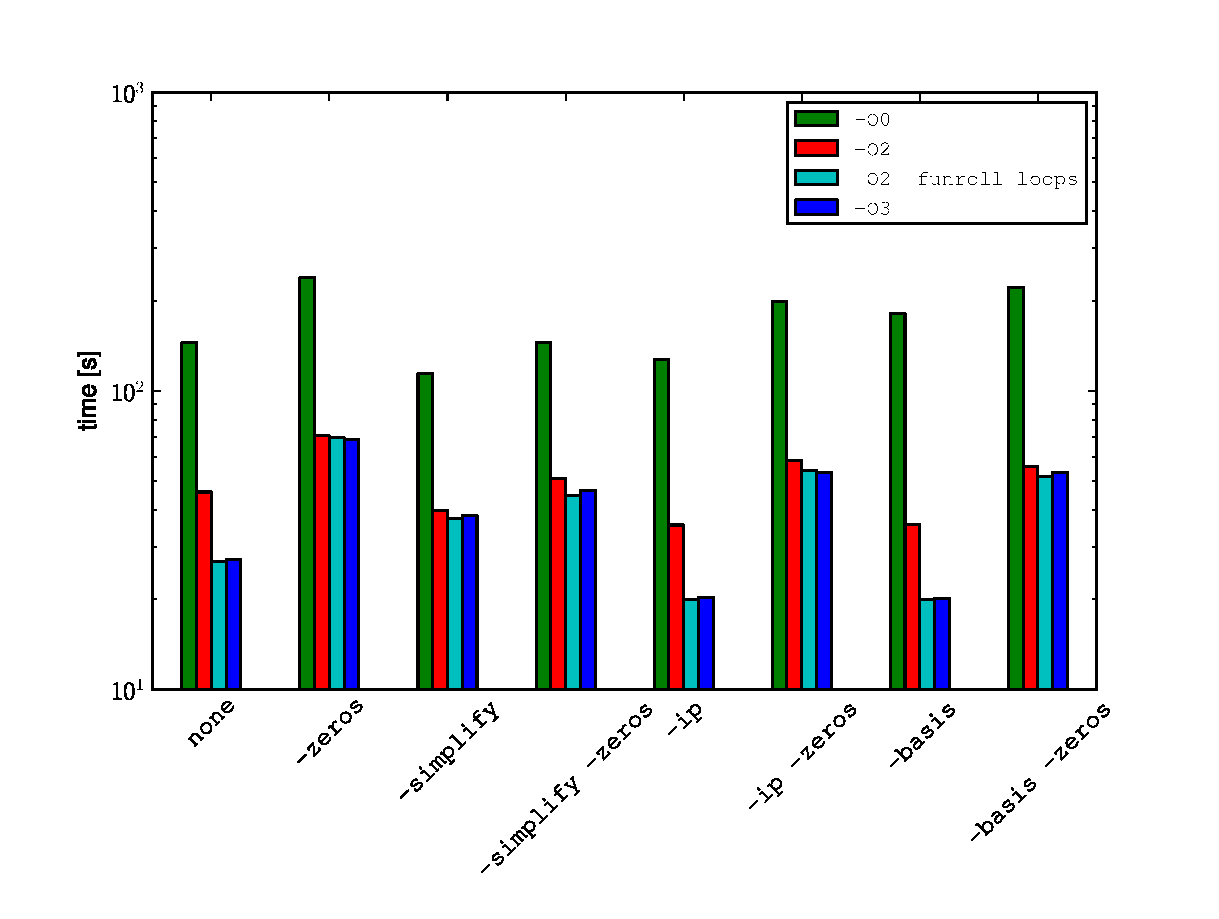
\includegraphics[width=0.8\textwidth]{chapters/oelgaard-2/pdf/runtime_laplace.pdf}
  \end{center}
  \caption{Runtime performance for the weighted Laplace equation for different
           compiler options.}
  \label{oelgaard-2:fig:laplace_stats_2}
\end{figure}
%
The \ffc{} and \emp{g++} compile times were less than one second for all
optimisation options.
It is clear from the figure that runtime performance is greatly influenced by
the \emp{g++} optimisations.
Compared to the case where no \emp{g++} optimisations are used, the runtime for
the standard quadrature code improves by a factor of 3.15 when using the
\emp{-O2} option and 5.40 when using the \emp{-O2 -funroll-loops} option.
The \emp{-O3} option does not appear to influence the runtime noticeably,
and if anything the performance decreases with this optimisation level.
Using the \ffc{} optimisation option \emp{-zeros} alone for this
form does not improve runtime performance.
In fact, using this option in combination with any of the other
optimisation options increases
the runtime, even when combining with the option \emp{-simplify}, which has a
significant lower operation count compared to the standard quadrature
representation.
A curious point to note is that without \emp{g++} optimisation (the \emp{-O0} flag)
there is a significant
difference in runtime for the \emp{-ip} and \emp{-basis} options, even though they
involve the same number of flops.
When \emp{g++} optimisations are switched on, this difference is eliminated
completely and the runtime for the two \ffc{} optimisations are identical.
This suggests that it is impossible to predict runtime performance from the
operation count alone since the type of \ffc{} optimisation must be taken into
account as well as the intended use of \emp{g++} compiler options.
The optimal combination of optimisations for this form is \ffc{} optimisation
\emp{-ip} or \emp{-basis} combined with the \emp{g++} option \emp{-O2}, in which
case the runtime has improved by a factor of 7.23 compared to standard
quadrature code with no \emp{g++} optimisations.

The operation counts and \ffc{} compile time for the bilinear form for
hyperelasticity with different \ffc{} optimisations are presented in
Table~\ref{oelgaard-2:tab:hyper_stats_1} while
Figure~\ref{oelgaard-2:fig:hyper_stats_2} shows the runtime performance for
different \emp{g++} compiler options for $N = 1 \times 10^4$.
%
\begin{table}
\caption{\ffc{} compile times and operation counts for the hyperelasticity example.}
\label{oelgaard-2:tab:hyper_stats_1}
\begin{center}\small
\begin{tabular}{l|rr|rr}
\multicolumn{1}{c}{\ffc{}}       & \multicolumn{2}{c}{\ffc{} time} & \multicolumn{2}{c}{} \\
\multicolumn{1}{c}{optimisation} & {\scriptsize [s]} & o/q         & flops     & o/q      \\
\hline
\emp{None}                       &  8.1              & 1.00        & 136531980 & 1.000 \\
\emp{-zeros}                     &  8.3              & 1.02        &  60586218 & 0.444 \\
\emp{-simplify}                  & 22.3              & 2.75        &   5950646 & 0.044 \\
\emp{-simplify -zeros}           & 21.2              & 2.62        &    356084 & 0.003 \\
\emp{-ip}                        & 15.2              & 1.88        &  90146710 & 0.660 \\
\emp{-ip -zeros}                 & 17.9              & 2.21        &  14797360 & 0.108 \\
\emp{-basis}                     & 15.2              & 1.88        &   7429510 & 0.054 \\
\emp{-basis -zeros}              & 17.8              & 2.20        &   1973521 & 0.014
\end{tabular}
\end{center}
\end{table}
%
\begin{figure}
  \begin{center}
    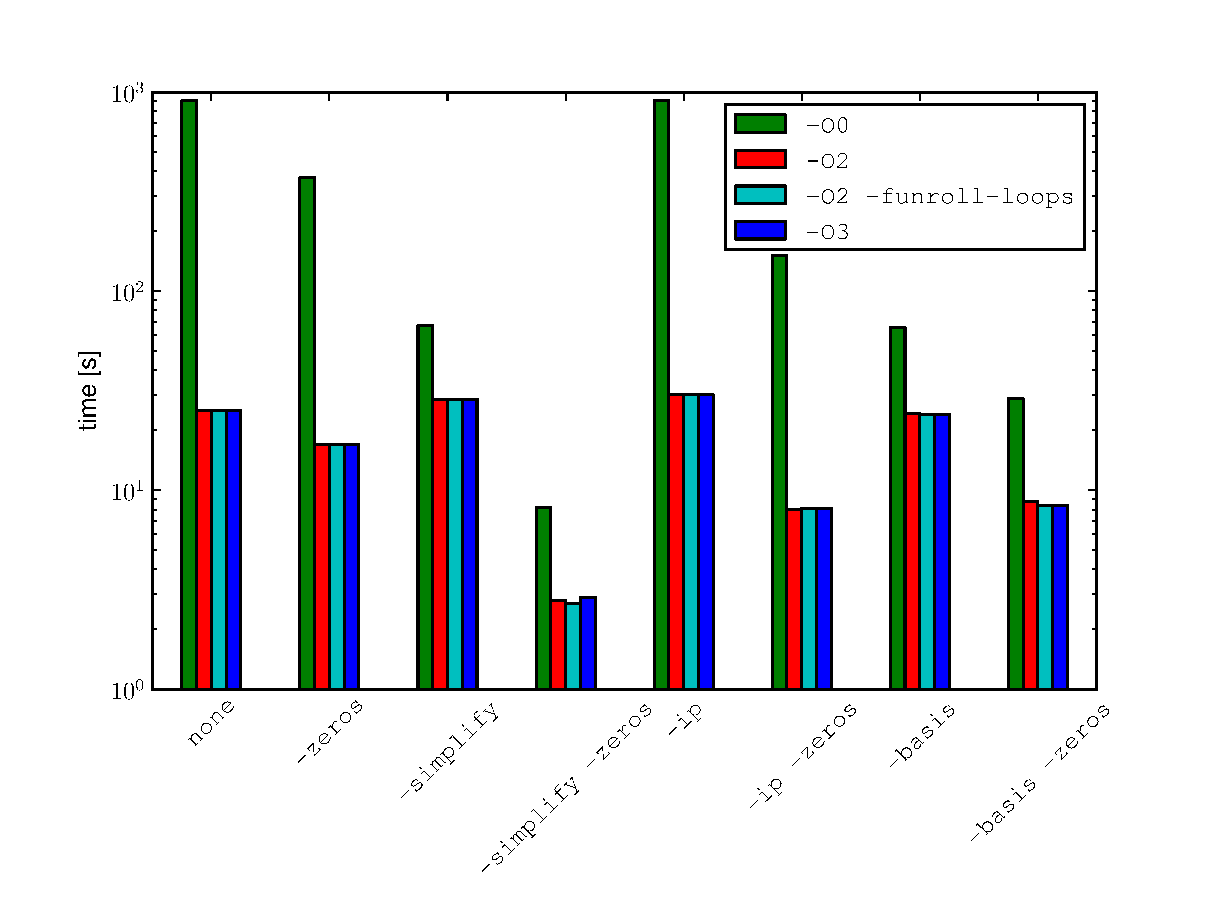
\includegraphics[width=0.8\textwidth]{chapters/oelgaard-2/pdf/runtime_hyperelasticity.pdf}
  \end{center}
  \caption{Runtime performance for the hyperelasticity example for different
           compiler options.}
  \label{oelgaard-2:fig:hyper_stats_2}
\end{figure}
%
Comparing the number of flops involved to the weighted Laplace example,
it it clear the this problem is considerably more complex.
The \ffc{} compile times in Table~\ref{oelgaard-2:tab:hyper_stats_1} show
that the \emp{-simplify} optimisation, as anticipated, is the most expensive to
perform.
The \emp{g++} compile times for all test cases were in the range two to six
seconds for all optimisation options.
A point to note is that scope for reduction in the flops count is considerably
greater for this problem than for the weighted Laplace problem,
with a difference in the number of flops spanning
several orders of magnitude between the different \ffc{} optimisations.
This compares to a reduction in flops of roughly two between
the non-optimised and the most effective optimisation strategy for the
weighted Laplace problem.
In the case where no \emp{g++} optimisation is used the runtime performance
for the hyperelastic problem
can be directly related number of floating point operations.
When the \emp{g++} optimisation \emp{-O2} is switched on, this effect becomes
less pronounced.
Another point to note, in connection with the \emp{g++} optimisations, is that
switching on additional optimisations beyond \emp{-O2}
does not seem to have an effect on the runtime.
For the hyperelasticity example, the option \emp{-zeros} has a positive effect
on the performance, both when used alone but in particular when combined with
the other \ffc{} optimisations.
This is completely opposite of what was the case for the weighted Laplace
equation the reason being that the test and trial functions are vector valued
rather than scalar valued which allows more zeros to be eliminated.
Finally, it is noted that the \emp{-simplify} option performs particularly well
for this example compared to the weighted Laplace problem.
The reason is that the nature of the hyperelasticity form results in a
relatively complex expression to compute the entries in the local element
tensor.
However, this expression only consists of a few different variables
(components of the inverse of the Jacobian and basis function values) which
makes the \emp{-simplify} option very efficient since a lot of terms are common
and can be precomputed and hoisted.
For the hyperelasticity form the optimal combination of optimisations is \ffc{}
option \emp{-basis -zeros} and \emp{g++} option \emp{-O2 -funroll-loops} which
improves the runtime performance of the code by a factor of 3149 when compared
to the case where no optimisation is used by either \ffc{} or~\emp{g++}.

For the considered examples, it is clear that no one
optimisation strategy is the best for all cases.
Furthermore, the generation phase optimisations that one can best use
depends on which
optimisations are performed by the \emp{g++} compiler.
It is also very likely that different \emp{C++} compilers will give different
results for the test cases presented above.
The general recommendation for selecting the appropriate optimisation for
production code will therefore be that the choice should be based on a
benchmark program for the specific problem.
%
%------------------------------------------------------------------------------
\subsection{Relative performance of the quadrature and tensor representations}
\label{oelgaard-2:sec:performance_of_representations}
%
As demonstrated in the previous section, a given type of optimisation may
be effective for one class of forms, and be less effective
for another class of forms.
Similarly, differences can be observed between the quadrature and
tensor representations for different equations.
A detailed study on this issue was carried out in \citet{OlgaardWells2010}.
For convenience we reproduce here the main conclusions along with
Table~\ref{oelgaard-2:tab:elasticity2D_complex_comparison}, which has been
reproduced from the paper.
The results shown in this section pertain to an elasticity-like bilinear form
in two dimensions which is premultiplied by a number of scalar
coefficients~$f_{i}$:
%
\begin{equation}
  a\brac{\bm{v}, \bm{u}} = \int_{\Omega} (f_0 f_1, \ldots, f_{n_f} )\
  \nabla^s \bm{v} : \nabla^s \bm{u} \dx,
\label{oelgaard-2:eq:elasticity_form}
\end{equation}
%
where $n_f$ is the number of premultiplying coefficients.
The test and trial functions are denoted by $\bm{v}, \bm{u} \in V_{h}$, with
%
\begin{equation}
  V_{h} = \bracc{\bm{v} \in \brac{H^{1}\brac{\Omega}}^2: \ \bm{v}\vert_K \in \brac{P_{q}\brac{K}}^2
   \forall K \in \mathcal{T}}
\label{oelgaard-2:eq:elastictity_H1_vector_space}
\end{equation}
%
and the coefficient functions $f_{i} \in W_{h}$ with
%
\begin{equation}
  W_{h} = \bracc{f \in H^{1}\brac{\Omega}: \ f\vert_K \in P_{p}\brac{K}
   \forall K \in \mathcal{T}},
\label{oelgaard-2:eq:elasticity_H1_space}
\end{equation}
%
where $q$ and $p$ denote the polynomial order of the Lagrange basis functions.
The number of coefficients and the polynomial orders are varied and the number
of flops needed to compute the local element tensor is recorded for both
tensor and quadrature representations.
The results were obtained by using the optimisation options
`\emp{-f eliminate\_zeros -f simplify\_expressions}' for the quadrature
representation.
In Table~\ref{oelgaard-2:tab:elasticity2D_complex_comparison}
the flops for the tensor representation is presented together with the
ratio given by the flops for quadrature representation divided by the flops
for tensor representation, denoted by $q/t$.
In terms of flops, a ratio $q/t > 1$ indicates that the tensor representation is
more efficient and $q/t < 1$ indicates that the quadrature representation is
more efficient.
It was found that when comparing the runtime performance of the two
representations, the number of flops is a good indicator of which
representation will perform the best.
However, as we have shown in the previous section the quadrature code with the
lowest number of flops does not always perform best for a given form and
the runtime performance even depends on which \emp{g++} options are used.
This begs the question of whether or not it is possible to make a sound
selection between representations based only on an estimation of flops as
it was suggested in \citet{OlgaardWells2010}.
%
\begin{table}
\caption{The number of operations and the ratio between number of operations
         for the two representations for the elasticity-like tensor in two
         dimensions as a function of different polynomial orders and numbers of
         functions.}
\label{oelgaard-2:tab:elasticity2D_complex_comparison}
\begin{center}\small
\begin{tabular}{l|rr|rr|rr}
\multicolumn{1}{c}{} & \multicolumn{2}{c}{$n_f = 1$} & \multicolumn{2}{c}{$n_f = 2$} & \multicolumn{2}{c}{$n_f = 3$}\\
                  & flops & q/t          & flops & q/t          & flops & q/t\\
\hline
$p = 1$, $q = 1$  &    888  &  0.34               &    3060 &  0.36               &   10224 & 0.11\\
$p = 1$, $q = 2$  &   3564  &  1.42               &   11400 &  1.01               &   35748 & 0.33\\
$p = 1$, $q = 3$  &  10988  &  3.23               &   34904 &  1.82               &  100388 & 0.63\\
$p = 1$, $q = 4$  &  26232  &  5.77               &   82548 &  2.87               &  254304 & 0.93\\
\hline
$p = 2$, $q = 1$  &    888  &  1.20               &    8220 &  0.31               &   54684 & 0.09\\
$p = 2$, $q = 2$  &   7176  &  1.59               &   41712 &  0.49               &  284232 & 0.11\\
$p = 2$, $q = 3$  &  22568  &  2.80               &  139472 &  0.71               &  856736 & 0.17\\
$p = 2$, $q = 4$  &  54300  &  4.36               &  337692 &  1.01               & 2058876 & 0.23\\
\hline
$p = 3$, $q = 1$  &   3044  &  0.36               &   30236 &  0.16               &  379964 & 0.02\\
$p = 3$, $q = 2$  &  12488  &  0.92               &  126368 &  0.26               & 1370576 & 0.03\\
$p = 3$, $q = 3$  &  36664  &  1.73               &  391552 &  0.37               & 4034704 & 0.05\\
$p = 3$, $q = 4$  &  92828  &  2.55               &  950012 &  0.49               & 9566012 & 0.06\\
\hline
$p = 4$, $q = 1$  &   3660  &  0.68               &   73236 &  0.11               & 1275624 & 0.01\\
$p = 4$, $q = 2$  &  17652  &  1.16               &  296712 &  0.16               & 4628460 & 0.02\\
$p = 4$, $q = 3$  &  57860  &  1.71               &  903752 &  0.22               &13716836 & 0.02\\
$p = 4$, $q = 4$  & 138984  &  2.46               & 2133972 &  0.29               &32289984 & 0.03
\end{tabular}
\end{center}
\end{table}
%
Nevertheless, some general trends can still be read from the table.
Increasing the number for coefficient functions $n_f$ in the form clearly
works in favour of quadrature representation.
For $n_{f}=3$ the quadrature representation can be expected to perform best for
all values of $q$ and~$p$.
Similarly, the difference in flops decreases when the polynomial order of the
coefficients, $p$, is increased although the effect is less pronounced compared
to the effect of increasing the number of coefficients.
The tensor representation appears to perform better when the polynomial order
of the test and trial functions, $q$, is increased although the effect is most
pronounced when the number of coefficients is low.
%
%------------------------------------------------------------------------------
\section{Automatic selection of representation}
%
We have illustrated how the runtime performance of the
generated code for variational forms can be improved by using various
optimisation options for the \ffc{} and \emp{g++} compilers and even by
changing the representation of the form.
Choosing the combination of form representation and optimisation options that
leads to optimal performance will inevitably require a benchmark study of the
specific problem.
However, very often many variational forms of varying complexity are needed to
solve more complex problems and setting up benchmarks for all of them is
cumbersome and time consuming.
Additionally, during the model development stage runtime performance is of
minor importance compared to rapid prototyping of variational forms as long as
the generated code performs reasonably well.

The default behaviour of \ffc{} is therefore to automatically determine which
form representation should be used based on a measure for the cost of using
tensor representation.
In short the cost is simply computed as the maximum value of the sum of the
number of coefficients and derivatives present in the monomials representing
the form.
If this cost is larger than a specified threshold, currently set to three,
quadrature representation is selected.
Recall from Table~\ref{oelgaard-2:tab:elasticity2D_complex_comparison} that
when $n_f=3$ the flops for quadrature representation was significantly lower
for virtually all the test cases.
Although this approach may seem \emph{ad hoc}, it will work well for those
situations where the difference in runtime performance is significant.
It is important to remember that the generated code is only concerned with the
evaluation of the local element tensor and that the time needed to insert the
values into a sparse matrix and to solve the system of equations will
reduce any difference, particularly for simple forms.
Therefore, making a correct choice of representation is less important for
forms where the difference in runtime performance is small.
A future improvement could be to devise a strategy for also letting the system
automatically select the optimisation strategy, for quadrature representation,
which is most likely to perform best.
%------------------------------------------------------------------------------

